\documentclass[10pt]{beamer}
%\documentclass[10pt, handout]{beamer}
\setbeameroption{show notes}

%\documentclass[10pt, a4paper]{article}
%\usepackage{beamerarticle}




\mode<article>{
	
	\usepackage{hyperref}
	
}
\mode<presentation>{
	
	\usetheme{Antibes}
	\usefonttheme{professionalfonts} 
	\usefonttheme{serif} % default family is serif
	
	%\usecolortheme{spruce} %зеленая, плохой цвет в заголовках 
	%\usecolortheme{albatross} %синяя, пхоло виден черный цвет
	
}

\newcommand{\MP}[1]{\mode<presentation>{#1} }
\newcommand{\MA}[1]{\mode<article>{#1} }

\newcommand{\ABS}[1]{\left| #1 \right|}
%\newcommand{\ABS}[1]{\mid #1 \mid}

\newcommand{\HREF}[2]{{\color{blue}\underline{\href{#1}{#2}}}}

\setbeamertemplate{caption}[numbered]


%\usepackage[T2A]{fontenc}
%\usepackage[utf8]{inputenc}
%\usepackage[russian]{babel}
%\usepackage{amsmath} %математические формулы



\usepackage{ifthen}

\usepackage{tikz}
\usetikzlibrary{arrows.meta}
\usetikzlibrary{calc}
\usetikzlibrary{decorations}
\usetikzlibrary{decorations.pathreplacing}
\newcommand{\rememb}[1]{\tikz[remember picture,baseline=-0.5ex]{\draw node[inner sep=0pt, outer sep=0pt] (#1){\strut};}}



\usepackage{fp}
\usepackage{tikz-3dplot}
\usepackage{environ}
\usepackage{animate}





\usepackage{xcolor}
%\usepackage[left=20mm,right=20mm,top=20mm,bottom=20mm,a4paper]{geometry} %поля

\usepackage{amsmath} %математические формулы
%\usepackage{amsfonts} %математические шрифты


\usepackage[e]{esvect}  %Красивая стрелочка вектора
%\let\oldvv\vv
\newcommand{\VV}[1]{\vv{#1\mathstrut}}



\usepackage{graphicx} %работа с каритнками


%\usepackage{multimedia}
%\usepackage{movie15}

%Для XeLatex/+
\usepackage{polyglossia}
\setdefaultlanguage{russian}
\setotherlanguage{english}
%\setkeys{russian}{babelshorthands=true} 


\usepackage{fontspec}

\setmainfont{Times New Roman} [Script=Cyrillic, Mapping=tex-text,]
\setsansfont{Arial} [Script=Cyrillic, Mapping=tex-text,]
%\setmonofont{Courier New} [Script=Cyrillic, Mapping=tex-text,]
\newfontfamily{\cyrillicfonttt}{Courier New}


%\usepackage{unicode-math}
%\setmathfont{TeX Gyre Termes Math}

%\setmainfont{CMU Serif}[Script=Cyrillic, Mapping=tex-text,]
%\setsansfont{CMU Sans Serif}[Script=Cyrillic, Mapping=tex-text,]
%\setmonofont{CMU Typewriter Text}[Script=Cyrillic, Mapping=tex-text,]


%-----------------


%\usepackage{caption}
%\DeclareCaptionLabelSeparator{dot}{~---~}            %Разделитель номер рисунка
%\captionsetup[figure]{justification=centering,labelsep=dot, format=plain}                        %Подпись рис. центр
%\captionsetup[table]{justification=raggedleft,labelsep=dot, format=plain, singlelinecheck=false} %Подпись табл. слева
%\captionsetup[lstlisting]{justification=raggedleft,labelsep=dot, format=plain, singlelinecheck=false}                     %Подпись рис. центр

\usepackage{indentfirst} %отступ первой строки


\usepackage[svgnames]{xcolor}


\usepackage{hyperref}

%\usepackage{showframe}


%\usepackage{tikz}

%\usepackage[hidelinks]{hyperref}%ссылки внутри документа \ref


\setlength\abovecaptionskip{-2pt}
%\setlength\belowcaptionskip{-14pt}

\setbeamerfont{caption}{size=\scriptsize}


\def\sectionname{Раздел}
\def\subsectionname{Подраздел}


\newcommand{\TC}[3]
{
	
	
	\begin{columns}
		\begin{column}{#1\textwidth}
			#2
		\end{column}
		\begin{column}{\fpeval{1-#1}\textwidth}
			#3
		\end{column}
	\end{columns}
}

\newcommand{\TCT}[3]
{
	
	\begin{columns}[T]
		\begin{column}{#1\textwidth}
			#2
		\end{column}
		\begin{column}{\fpeval{1-#1}\textwidth}
			#3
		\end{column}
	\end{columns}
}


\newcommand{\FRAME}[2]{
	\begin{frame}
		\frametitle{#1}
		#2
	\end{frame}
}

\newcommand{\FIG}[3]
{
	\begin{figure}
		\centering
		\includegraphics[width=#3]{#1}
		\caption{#2}
	\end{figure}
}

\newcommand{\vect}[1]{\overrightarrow{#1}}


\usepackage{qrcode}

\newcommand{\LECADDR}{https://clck.ru/3D3Efj}


\usepackage{newfile}

\edef\LectionNumber{0}
\edef\LectionTheme{0}

\let\oldsection\section
\let\oldsubsection\subsection


\AtBeginDocument
{
	\newoutputstream{CONTENT}
	\openoutputfile{\LectionNumber .gvr}{CONTENT}
	
	\expandafter\addtostream{CONTENT}{\noindent\textbf{\Large Лекция \LectionNumber~---~\LectionTheme}\unexpanded{\setcounter{SEC}{0}}\par}
}

\renewcommand{\section}[1]{
	\oldsection{#1}
	\expandafter\addtostream{CONTENT}{\noindent\hspace{2ex}\unexpanded{\hbox{\large\stepcounter{SEC}\theSEC ~ #1}}\par}
}

\renewcommand{\subsection}[1]{
	\oldsubsection{#1}
	\expandafter\addtostream{CONTENT}{\noindent\hspace{6ex}\unexpanded{\stepcounter{SUB}\theSUB ~ #1}\par}
}


%\renewcommand{\section}[1]{\MMM{#1}}

%\edef\subsection#1
{
	%\noexpand\subsection{#1}
	%
}


\newfontfamily\dnifamily[Scale = 0.795]{DniFont.TTF}

\newcommand{\dni}[1]{%
	{\dnifamily%
		\ifthenelse{#1=0}{0}{}%
		\ifthenelse{#1=1}{1}{}%
		\ifthenelse{#1=2}{2}{}%
		\ifthenelse{#1=3}{3}{}%
		\ifthenelse{#1=4}{4}{}%
		\ifthenelse{#1=5}{5}{}%
		\ifthenelse{#1=6}{6}{}%
		\ifthenelse{#1=7}{7}{}%
		\ifthenelse{#1=8}{8}{}%
		\ifthenelse{#1=9}{9}{}%
		\ifthenelse{#1=10}{)}{}%
		\ifthenelse{#1=11}{!}{}%
		\ifthenelse{#1=12}{@}{}%
		\ifthenelse{#1=13}{\#}{}%
		\ifthenelse{#1=14}{\$}{}%
		\ifthenelse{#1=15}{\%}{}%
		\ifthenelse{#1=16}{\^{}}{}%
		\ifthenelse{#1=17}{\&}{}%
		\ifthenelse{#1=18}{*}{}%
		\ifthenelse{#1=19}{(}{}%
		\ifthenelse{#1=20}{[}{}%
		\ifthenelse{#1=21}{]}{}%
		\ifthenelse{#1=22}{\textbackslash{}}{}%
		\ifthenelse{#1=23}{\{}{}%
		\ifthenelse{#1=24}{\}}{}%
		\ifthenelse{#1=25}{|}{}}%
}%

\newcommand{\toDni}[1]{%	
	\ifthenelse{#1=0}{}{%
		 \ifthenelse{#1=25}{%
		 	\expandafter\dni{#1}}{%
		 	\expandafter\toDni{\fpeval{floor(#1/25)}}%
		 \expandafter\dni{\fpeval{(#1/25 - floor(#1/25))/0.04}}}}%
}%



\newcommand{\Strut}{{\Large\strut}}

\newcommand\scb[1]{\left( #1 \right)}

\newcommand{\LINK}[2]{%
	\qrcode[height=1cm]{#1}\  \HREF{#1}{\parbox{0.8\textwidth}{#2}} \\[0.5em]
}

\NewDocumentCommand{\lecdni}{}{\toDni{\LectionNumber}}
\author{Гаврилов Андрей Геннадьевич}
\newcommand{\regals}{кандидат технических наук, доцент}
\institute{Кафедра Информационных технологий и вычислительных систем \\МГТУ~<<СТАНКИН>>}
\lecture{История компьютерной графики}{kghistory}\subtitle{Компьютерная графика}


\makeatletter
\newcommand*{\overlaynumber}{\number\beamer@slideinframe}
\makeatother



\usepackage{cprotect}

\newcommand{\QRFRAME}{%
    \begin{frame}[plain, noframenumbering]    	
	
	\centering
	Трансляция презентации (во время очных лекций)    
	
	~
	
	{\Large \ttfamily  https://clck.ru/3D3Efj  }
	
	~
	
	\tikz\node[inner sep=0pt,rounded corners=5mm, clip]{\qrcode[height=0.45\textwidth]{\LECADDR}}; 
	
	~	
	{\small
	При просмотре презентации в PDF для отображения анимаций на слайдах необходимо использовать Acrobat Reader, KDE Okular, PDF-XChange, Foxit Reader, браузер Firefox. Для браузеров на движке Chrome (Edge, Яндекс, Opera,~\dots) необходимо использовать \HREF{https://chromewebstore.google.com/detail/pdf-viewer/oemmndcbldboiebfnladdacbdfmadadm?hl=ru&utm_source=ext_sidebar}{PDF.js} c опцией <<Enable active content (JavaScript) in PDFs>>. }
	
	\end{frame}%
}

\newcommand{\IG}[2][1]{\includegraphics[width=#1\textwidth]{#2}}



\graphicspath{{Images/}{Images/\jobname/}}

\date{\today}



\renewcommand{\LectionNumber}{6}
\renewcommand{\LectionTheme}{Отсечение отрезков и растеризация}
\title{Лекция \lecdni \\ \LectionTheme}
\subtitle{Компьютерная графика}



%\usepackage{standalone}

\setbeamersize
{
	text margin left=0.5cm,
	text margin right=0.5cm
}

\usepackage{comment}


%	\transduration{2}
%   \transfade

 \begin{document}
 		 
	\makeatletter
\defbeamertemplate*{title page}{my theme}
{
	
	\hfill
	
	\begin{beamercolorbox}[wd=.9\paperwidth,center,]{title}%
		
	\end{beamercolorbox}%	
	
	\vbox to 1em {}
	
	\begin{beamercolorbox}[wd=.9\paperwidth,center,]{title}%
		\usebeamerfont{subtitle}%
		\hfill
		
		\insertsubtitle
		
		\usebeamerfont{title}%
		\inserttitle{} \\[0.5em]
		
		
		
	\end{beamercolorbox}%	
	\hfill\hfill
	
	\begin{beamercolorbox}[wd=.9\paperwidth,center,]{}%
		\usebeamerfont{author}%
		\hfill \\[0.5em]
		\insertauthor{} \\[0.5em]
		\regals
		    
		\vbox to 1em{}
		\usebeamerfont{institute}%
		\insertinstitute {}
		
		\vbox to 1em{}			
		{\; }\insertshortdate{}
		
	\end{beamercolorbox}%	
	\hfill\hfill
	
	\vbox to 5em{}
	
	
}
\defbeamertemplate*{footline}{my theme}{
	\leavevmode%
	\hbox{%
		\begin{beamercolorbox}[wd=.25\paperwidth,ht=3.25ex,dp=0ex,center,sep=1pt]{author in head/foot}%
			\usebeamerfont{author in head/foot}%
			\insertauthor 
			\beamer@ifempty{\insertshortinstitute}{}
		\end{beamercolorbox}%
		\begin{beamercolorbox}[wd=.65\paperwidth,ht=3.25ex,dp=0ex,center,sep=1pt]{title in head/foot}%
			\usebeamerfont{title in head/foot}\insertshortinstitute
		\end{beamercolorbox}%
		\begin{beamercolorbox}[wd=.1\paperwidth,ht=3.25ex,dp=0ex,center, sep=0.5pt]{date in head/foot}%
			\usebeamerfont{date in head/foot}
			\footnotesize \expandafter\toDni{\insertframenumber} / \expandafter\toDni{\inserttotalframenumber}
	\end{beamercolorbox}}%
}



\makeatother






%float page top aligment
\makeatletter
\setlength{\@fptop}{0pt}
\setlength{\@fpbot}{0pt plus 1fil}
\makeatother

\newcommand \abs[1] {\left| #1 \right|}

%\everymath{\displaystyle}

\begin{comment}
\end{comment}

    
    \QRFRAME	
	
	
	\frame{\maketitle}
	
	
	
	\begin{frame}{План лекции}
		\tableofcontents
	\end{frame}
	

	
	\section{Отчесение отрезков}	
	\frame{\sectionpage}
	
	
	\begin{frame}{Постановка задачи}
		
		\begin{center}
			\TC{0.55}
			{
				\includegraphics[page=1]{line_slise.pdf}
			}
			{
				~ \\
				
				1 --- отрисуется полностью
				
				2 --- $AB \rightarrow (AP, PB)$ 
				
				\ \ $AB$ --- отрисуется,
				
				\ \ $PB$ --- отбрасывается
				
				
				3 --- должен быть отброшен
			
			}
			
		\end{center}
		
		$\dfrac{B_y-A_y}{B_x-A_x} = \dfrac{P_y-A_y}{P_x-A_x}$
		~$\Rightarrow$~ 
		\fbox {$ P_x = \dfrac{B_x-A_x}{B_y-A_y}(y_{max}-A_y)+A_x 	$}
		

		
		
	\end{frame}
	
	
	\subsection{Алгоритм Коэна-Сазерленда}		
	
    \frame{\subsectionpage}
	
	\begin{frame}{Алгоритм Коэна-Сазерленда}
		
		\TCT{0.55}
		{
			\includegraphics[page=1]{koen-saz.pdf}
		}{
				4х битный код  ${\color{Red}b_0}{\color{Green}b_1}{\color{Blue}b_2}{\color{Fuchsia}b_3}$:
		
		
				$
				{\color{Red}b_0}= \begin{cases}
					0, & x \geq x_{min} \\
					1, & x < x_{min} \\
				\end{cases}
				$ 
				
				$
				{\color{Green}b_1}= \begin{cases}
					0, & x \leq x_{max} \\
					1, & x > x_{max} \\
				\end{cases}
				$ 
				
				$
				{\color{Blue}b_2}= \begin{cases}
					0, & y \geq y_{min} \\
					1, & y < y_{min} \\
				\end{cases}
				$  
				
				$
				{\color{Fuchsia}b_3}= \begin{cases}
					0, & y \leq y_{max} \\
					1, & y > y_{max} \\
				\end{cases}
				$  
		}
		
	\end{frame}
	
	
	
	\begin{frame}{Тривиальные случаи}

		
			\begin{center}
				\includegraphics[page=2]{koen-saz.pdf}
			\end{center}
			
			1: Побитовое ИЛИ кодов концов отрезка == 0 --- отрезок видим ($\odot$).
			
			2 и 3: Побитовое И концов отрезка == 1 --- отрезок не видим($\otimes$).
			
			В остальных ситуациях ($\circledast$) требуется сведение к $\odot$ или  $\otimes$.
		
		
		
	\end{frame}
	
	\begin{frame}{Нетривиальные случаи (1)}
		\TC{0.6}{
			\only<1>{\includegraphics[page=3]{koen-saz.pdf}
			}\only<2->{\includegraphics[page=4]{koen-saz.pdf}}
			}
		{
			$A=0001, \ B=0000$
			
			$ A\vee B \neq 0,\ A \wedge B = 0$ --- $\circledast$. \footnotemark \\ ~ \\
			
			\pause
			
			$A \rightarrow P, \ P = 0000$ 
			
					
			$B \vee P = 0$ --- $\odot$
		}
		
		\footnotetext[1]{$\wedge$ --- конъюнкция, логическое И, умножение	\\		
			\ \ \ \ \ \ \	$\vee$ --- дизъюнкция, логическое ИЛИ, сложение}
	\end{frame}
	
	
	\begin{frame}{Нетривиальный случай (2)}
		\TC{0.62}
		{
			\only<1>{\includegraphics[page=5]{koen-saz.pdf}
			}\only<2>{\includegraphics[page=6]{koen-saz.pdf}
			}\only<3>{\includegraphics[page=7]{koen-saz.pdf}
			}
		}
		{
			$A = 0101, \ B=0010$ 
			
			$A \vee B \neq 0, \ A \wedge B = 0$ --- $\circledast$ \\ ~ \\
			
			\pause
			
			$A \rightarrow A_1, A_1 = 0000$
			
			$A_1 \vee B \neq 0, \ A_1 \wedge B = 0$ --- $\circledast$ \\ ~ \\
			
			\pause
			
			$B \rightarrow B_1, B_1 = 0000$
			
			$A_1 \vee B_1 = 0$ --- $\odot$.
			
		}
	\end{frame}
	
	
	\begin{frame}{Нетривиальный случай (3)}
		\TC{0.5}
		{
			\only<1>{\includegraphics[page=8]{koen-saz.pdf}
			}\only<2>{\includegraphics[page=9]{koen-saz.pdf}
			}\
		}
		{
			$A = 0010, \ B=1001$ 
			
			$A \vee B \neq 0, \ A \wedge B = 0$ --- $\circledast$ \\ ~ \\
			
			\pause
			
			$A \rightarrow A_1, A_1 = 1000$
			
			$A_1 \vee B \neq 0, \ A_1 \wedge B = 1$ --- $\otimes$ \\ ~ \\
			
			
		}
		
	\end{frame}
	
	\begin{frame}{Нетривиальный случай (4)}
		\TC{0.5}
		{
			\only<1>{\includegraphics[page=10]{koen-saz.pdf}
			}\only<2>{\includegraphics[page=11]{koen-saz.pdf}
			}\only<3>{\includegraphics[page=12]{koen-saz.pdf}
			}\only<4>{\includegraphics[page=13]{koen-saz.pdf}
			}
		}
		{
			$A = 1010, \ B=0001$ 
			
			$A \vee B \neq 0, \ A \wedge B = 0$ --- $\circledast$ \\ ~ \\
			
			\pause
			
			$A \rightarrow A_1, A_1 = 0010$
			
			$A_1 \vee B \neq 0, \ A_1 \wedge B = 0$ --- $\circledast$ \\ ~ \\
			
			
			\pause
			
			$A_1 \rightarrow A_2, A_2 = 0000$
			
			$A_2 \vee B \neq 0, \ A_2 \wedge B = 0$ --- $\circledast$ \\ ~ \\
			
			\pause
			
			$B \rightarrow B_1, B_1 = 0000$
			
			$A_2 \vee B_1 = 0$ --- $\odot$ \\ ~ \\
			
			
		}
		
	\end{frame}
	
	\subsection{Алгоритм средней точки}
	\frame{\subsectionpage}
	
	\begin{frame}{Алгоритм средней точки}
		
		\TC{0.4}
		{
			\foreach \fr in {1,2,3,4,5,6}{
			\only<\fr>{\includegraphics[page=\fr]{mid point.pdf}}
			}
			
			$(A,B)$ --- $\circledast$ \\ ~ \\
		}
		{
			
			\pause
			
			$P1 = \dfrac{A+B}{2}$ $\rightarrow$ $(A,P_1),(P_1,B)$
			
			$(A,P_1)$ --- $\circledast$ , $(P_1,B)$ --- $\circledast$ 	\\ ~ \\
			
			\pause
			
			$(A,P_1): \ P_2=\dfrac{P_1+A}{2}$
			
			$(A,P_2)$ --- $\otimes$,	$(P_1,P_2)$ --- $\circledast$ \\~\\
			
			\pause
			
			$(P_1,P_2): \ P_3=\dfrac{P_1+P_2}{2}$
			
			$(P_1,P_3)$ --- $\odot$,	$(P_3,P_2)$ --- $\circledast$ \\~\\
			
			\pause
			
			$(P_2,P_3): \ P_4=\dfrac{P_2+P_3}{2}$ \\
			
			\fbox{$P_4 \in x_{max}$}, $(P_4,P_2)$ --- $\otimes$, $(P_3,P_4)$ --- $\odot$	\\~\\
			
			\pause
			
			
			$(P_1,B) \rightarrow$  \fbox{$P_5 \in y_{min}$}
		}
		
	\end{frame}
	
	

	\subsection{Алгоритм Кируса-Бека}	
	\frame{\subsectionpage}
	
	\begin{frame}{Поиск пересечения отрезков}
		\TC{0.55}
		{
			\only<1>{\includegraphics[page=1]{cirus_case1.pdf}
			}\only<2>{\includegraphics[page=2]{cirus_case1.pdf}
			}\only<3->{\includegraphics[page=3]{cirus_case1.pdf}
			}	
		}
		{
			Дано: $\vv{AB}$, $f$: $(\vv n \perp f$, $F \in f)$ \\ ~ \\
			Найти: $\vv{AB} \cap f$ \\ ~ \\ \pause
			
			$AB \equiv P(t) = A + (B-A)t,$\\
			\hfill $ t \in [0, \dots, 1]$ \pause
		}
		
		$\VV{FP(t_1)}\cdot\VV n < 0$, \ \ $\VV{FP(t_3)}\cdot\VV n > 0$, \ \ $\VV{FP(t_2)}\cdot\VV n = 0$ \\[0.5em] \pause
		
		$(\VV{P(t)}-\VV{F})\cdot\vv n = 0$ \ $\Rightarrow$ \  $(\VV A+(\VV B-\VV A)t-\VV F)\cdot\VV n = 0$ \\[0.5em] \pause
		
		$(A-F)\cdot \VV n + (B-A)t \cdot \VV n = 0$  \ $\Rightarrow$ \  
		$t=-\dfrac{(\VV B-\VV A)\cdot\VV n}{(\VV A-\VV F)\cdot\VV n} =  \boxed{-\dfrac{(\VV{AB}\cdot\VV n )}{(\VV{FA}\cdot\VV n)} }$ 
		
				
		
	\end{frame}
	
	\begin{frame}{Направление выхода отрезка через сторону многоуг.}
		\TC{0.5}
		{
			\centering
			\includegraphics{cirus_case2.pdf}
			
			$\VV{AB}\cdot\VV n > 0 $, так как $\alpha \in \left( -\dfrac{\pi}{2},\dfrac{\pi}{2}\right)$ \\[0.5em]
			
			$\VV{BA}\cdot\VV n < 0 $, так как $\beta \in \left( \dfrac{\pi}{2},\dfrac{3\pi}{2}\right)$
		}
		{
			$f_i$ --- $i$-ая грань  многоугольника.
			
			$\vv n_i$ --- внутренняя нормаль к  $f_i$ \\ ~ \\
			
			$\VV{AB} \cdot \VV n_i = \abs{\VV{AB}} \abs{\VV n_i} \cos \widehat{\VV{AB}\,\VV n_i}={}$\\			
			\hfill $=\VV{AB}_x \VV{n_i}\,_x+\VV{AB}_y\VV{n_i}\,_y$ \\ ~ \\
			
			Если $\VV{AB} \cdot \VV n_i > 0$ --- $AB$ в\textbf{Х}одит через $f_i$ \\~\\
			Если $\VV{AB} \cdot \VV n_i < 0$ --- $AB$ в\textbf{Ы}ходит через $f_i$ \\ ~ \\
			Если $\VV{AB} \cdot \VV n_i = 0$ --- $AB \parallel f_i$ 
		}
	\end{frame}

	\begin{frame}{Алгоритм Кируса-Бека}
		\small
		
		\TC{0.65}
		{
			\foreach \fr in {1,2,...,11}{\only<\fr>{\includegraphics[page=\fr]{cirus.pdf}}}
			\pause
			$AB \equiv P(t) = A + (B-A)t, t \in [0, \dots, 1]$
			\begin{enumerate}
				\item<+-> $t_\text{вх}:=0, \ t_\text{вых}:=1$ 
				\item<+-> $\VV{AB}\cdot\VV n_1 < 0 \; \text{и} \; t \not< t_\text{вых}  \Rightarrow $ \\ $\Rightarrow t_\text{вых}\text{ не измен.} $
				\item<+-> $\VV{AB}\cdot\VV n_2 > 0 \; \text{и} \; t> t_\text{вх} \Rightarrow $ \\ $\Rightarrow t_\text{вх}:=t $
			\end{enumerate}
			
		}
		{
							
			\begin{enumerate}
				\setcounter{enumi}{4}
				\item<+-> $\VV{AB}\cdot\VV n_3 > 0 \; \text{и} \; t> t_\text{вх} \Rightarrow$ \\ $\Rightarrow t_\text{вх}:=t $
				\item<+-> $\VV{AB}\cdot\VV n_4 > 0 \; \text{и} \; t \not> t_\text{вх} \Rightarrow$ \\  $\Rightarrow t_\text{вх}\text{ не измен.} $
				\item<+-> $\VV{AB}\cdot\VV n_5 > 0 \; \text{и} \; t \not> t_\text{вх} \Rightarrow$ \\  $\Rightarrow t_\text{вх}\text{ не измен.} $
				\item<+-> $\VV{AB}\cdot\VV n_6 < 0 \; \text{и} \; t \not< t_\text{вых}  \Rightarrow$ \\  $\Rightarrow t_\text{вых}\text{ не измен.} $
				\item<+-> $\VV{AB}\cdot\VV n_7 < 0 \; \text{и} \; t < t_\text{вых}  \Rightarrow$ \\  $\Rightarrow t_\text{вых}:=t $
				\item<+-> $\VV{AB}\cdot\VV n_7 < 0 \; \text{и} \; t < t_\text{вых}  \Rightarrow$ \\  $\Rightarrow t_\text{вых}:=t $
				\item<+-> $t_\text{вх}<t_\text{вых} \Rightarrow$ \\
				 $\Rightarrow P(t_\text{вх})P(t_\text{вых}) $ --- $\odot$
			\end{enumerate}
		}
		
		
		
	\end{frame}

	
	\section{Алгоритмы растеризации}
	
	\frame{\sectionpage}
	
	\subsection{Цифровой дифференциальный анализатор}
	
	\begin{frame}{Алгоритм ЦДА (цифровой дифференциальный анализатор)}
		\TC{0.53}
		{
			\animategraphics[autoplay,loop,palindrome, nomouse]{15}{Images/\jobname/raster1}{0}{45}
		}
		{
			\small
			\begin{enumerate}
				\item<+-> $x_1:=\text{round}(A_x)$, $x_2:=\text{round}(B_x)$\\				
					  $y_1:=\text{round}(A_y)$, $y_2:=\text{round}(B_y)$\\
					  
					  
				\item<+-> $L:=\max(|x_2-x_1|,|y_2-y_1|)$
				
				\item<+-> $dx:=(x_2-x_1)/L$\\
				      $dy:=(y_2-y_1)/L$
				      
				\item <+->	$x:=x_1,\ y:=y_1$\\						
						$\text{for }i:=1 \text{ to } L$\\
						\quad $\text{draw}(\text{round}(x),\text{round}(y))$\\
						\quad $x:=x+dx$, $y:=y+dy$ \\
						
			\end{enumerate}
		}
	\end{frame}
	
	\subsection{Алгоритм Брезенхэма}
	
	\begin{frame}{Алгоритм Брезенхэма}
		\TC{0.52}
		{
			\animategraphics[autoplay,loop,palindrome, nomouse]{15}{Images/\jobname/raster2}{0}{45}
		}
		{
			\small
			\begin{center}
				\animategraphics[autoplay,loop, nomouse, width=0.7\textwidth]{1.5}{Images/\jobname/raster2.1}{0}{10}
			\end{center} ~\\[-3em]
			
			\begin{enumerate}
				\item<+-> 	$x_1:=\text{round}(A_x)$, $x_2:=\text{round}(B_x)$\\				
						$y_1:=\text{round}(A_y)$, $y_2:=\text{round}(B_y)$\\
						
				\item<+->  	$dx:=|x_2-x_1|, \ dy:=|y_2-y_1|$\\	
						$e:=0, \ de:=(dy+1)/(dx+1) $
						
						
				\item<+->  	$y:=y_1$\\
						$\text{for }x:=x_1\text{ to }x_2$\\
						\quad$\text{draw}(x,y)$\\
						\quad$e:=e+de$\\
						\quad $\text{if}(e \geq 1)\text{ then}$\\
						\quad\quad$y:=y+1$\\
						\quad\quad$e:=e-1$ 
			\end{enumerate}
		}
	\end{frame}
	
	\begin{frame}{ЦДА vs Брезенхэм}
		\centering
		\animategraphics[autoplay,loop,palindrome, nomouse]{15}{Images/\jobname/raster3}{0}{45}
		
	\end{frame}
	
	\subsection{Прочие алгоритмы}
	
	\begin{frame}{Алгоритм Ву}
		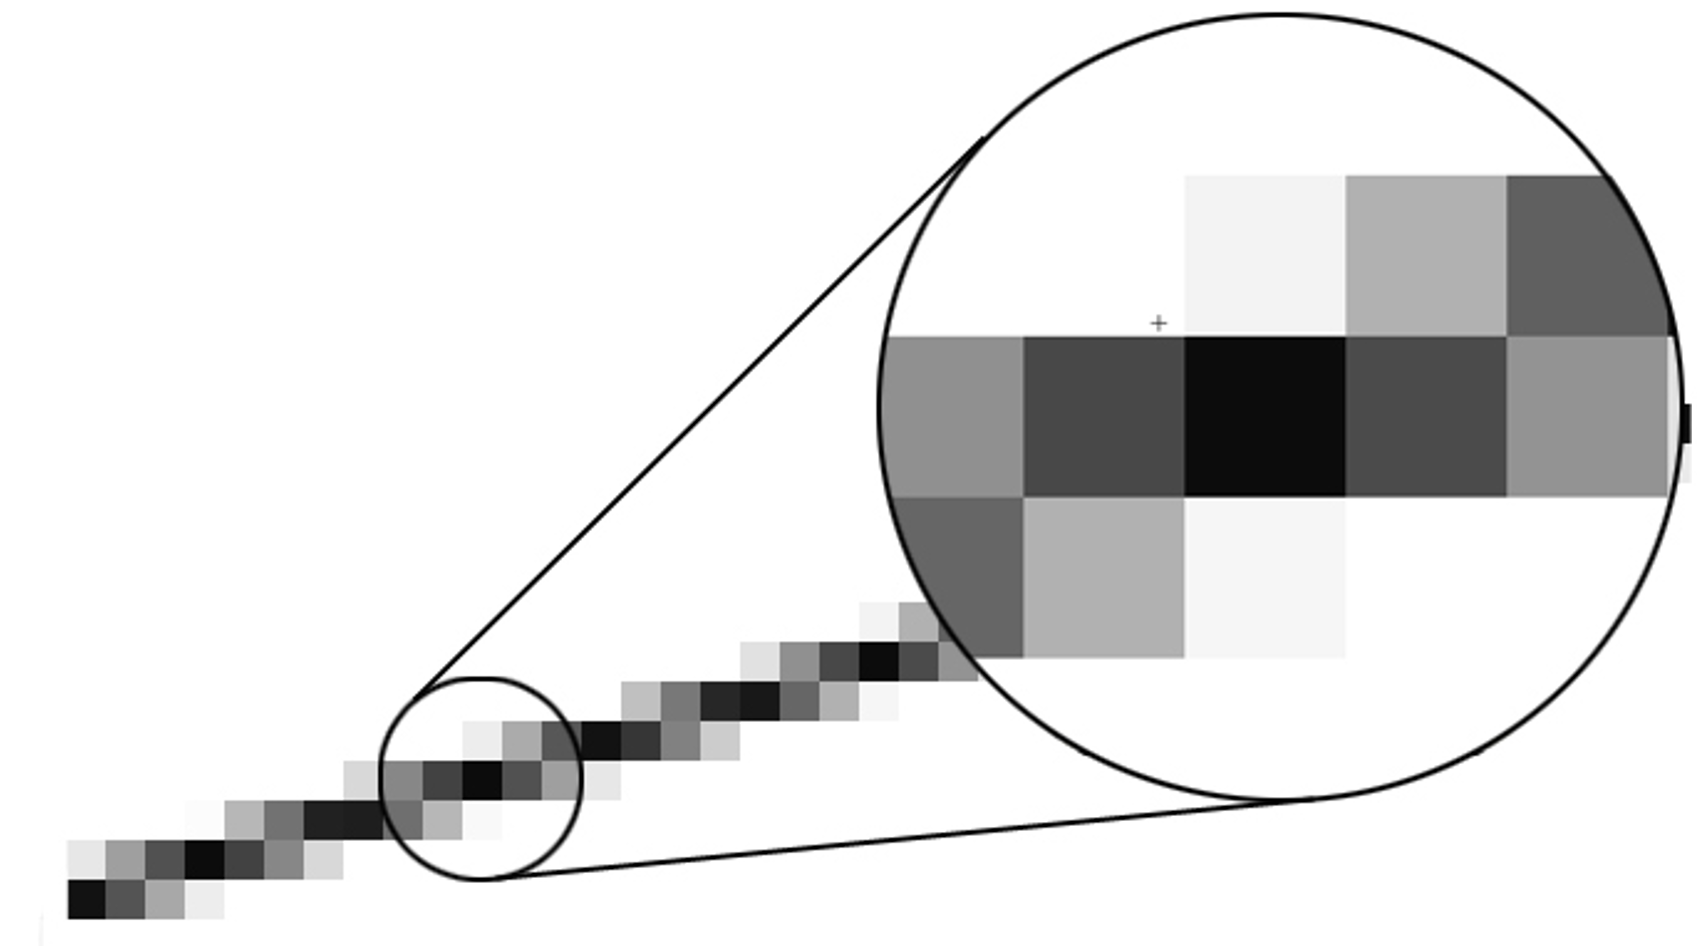
\includegraphics[width=\textwidth]{Screenshot 2024-05-04 011143.png}
	\end{frame}

\begin{comment}
\end{comment}

\end{document}